\documentclass{ieeeaccess}
\usepackage{cite}
\usepackage{amsmath,amssymb,amsfonts}
\usepackage{algorithmic}
\usepackage{graphicx}
\usepackage{textcomp}
\def\BibTeX{{\rm B\kern-.05em{\sc i\kern-.025em b}\kern-.08em
    T\kern-.1667em\lower.7ex\hbox{E}\kern-.125emX}}
\begin{document}
\history{Date of publication xxxx 00, 0000, date of current version xxxx 00, 0000.}
\doi{10.1109/ACCESS.2017.DOI}

\title{Bumper Car Sumo Proposal}
\author{\uppercase{First A. Author}\authorrefmark{1}, \IEEEmembership{Fellow, IEEE},
\uppercase{Second B. Author\authorrefmark{2}, and Third C. Author,
Jr}.\authorrefmark{3},
\IEEEmembership{Member, IEEE}}
\address[1]{National Institute of Standards and 
Technology, Boulder, CO 80305 USA (e-mail: author@boulder.nist.gov)}
\address[2]{Department of Physics, Colorado State University, Fort Collins, 
CO 80523 USA (e-mail: author@lamar.colostate.edu)}
\address[3]{Electrical Engineering Department, University of Colorado, Boulder, CO 
80309 USA}
\tfootnote{This paragraph of the first footnote will contain support 
information, including sponsor and financial support acknowledgment. For 
example, ``This work was supported in part by the U.S. Department of 
Commerce under Grant BS123456.''}

\markboth
{Author \headeretal: Preparation of Papers for IEEE TRANSACTIONS and JOURNALS}
{Author \headeretal: Preparation of Papers for IEEE TRANSACTIONS and JOURNALS}

\corresp{Corresponding author: First A. Author (e-mail: author@ boulder.nist.gov).}

\begin{abstract}
Americans aren’t having fun anymore. The weight of capitalism is forcing families to work 60 hour weeks for low, soul-crushing pay. So not only do Americans lack the time for fun, they often lack the funds as well, leading to inefficient forms of entertainment. People with low life satisfaction tend to be unproductive in both their social life and their work life. Not only does this result in reduced profits for businesses, but also creates a downward spiral in which people become increasingly devoid of enjoyment. To combat this atrocity, a new game is being developed that will fill the entertainment void that befall our fellow Americans. 
The cost and entertainment efficiency of our game will be the most important criteria for success. Costs should be low enough that most people can afford to play, while our game should yield high levels of fun per minute played. Because entertainment value is our primary goal, costs will only have a secondary role in our design process. Battle royale games have become a major hit in the entertainment world due to their competitive nature, as such our team decided to create a game where player-controlled robots attempt to push each other out of an arena. Last player remaining wins. To facilitate gameplay, our robots need to be easily pushed around by other robots. Games that drag on forever with little action are not fun. Controls should be easy to enhance playability, though not too easy as complexity adds to the fun. We need some way to detect game conditions, such as when a robot is out of bounds or when a player wins. This could be done with a human referee, but that would take away immersion of the game. Because some players may not have friends to play with, it is desirable to have some sort of AI to play against. Competitive games are much more enjoyable with worthy opponents.
Since cost is a contributing factor to our design, we will want to use existing technologies as much as possible. Robots can be constructed as a two-wheeled platform with wireless modules, similar to a segway. For extra entertainment, a spherical shell could encase the robot, reducing its traction on the play surface. A player’s phone can be used as a controller if a suitable app is developed. This negates the cost of constructing our own controllers at the slight cost of reduced playability. Computer vision libraries could allow us to track the location of each robot if painted differently. Exact positioning solves the problem of detecting game conditions, plus giving us plenty of information to use for a basic AI. 
Our goal, above all else, is that our game is fun. Playtesting will be a major component of our design process, rethinking aspects of the game if we decide it is not fun. Costs will be mitigated, but entertainment value will never be sacrificed for savings. Smiles and laughs from players is our primary measure of success.

\end{abstract}

\begin{keywords}
Enter key words or phrases in alphabetical 
order, separated by commas. For a list of suggested keywords, send a blank 
e-mail to keywords@ieee.org or visit \underline
{http://www.ieee.org/organizations/pubs/ani\_prod/keywrd98.txt}
\end{keywords}

\titlepgskip=-15pt

\maketitle

\section{Introduction}
\label{sec:introduction}
\PARstart{T}{his} document is a template for \LaTeX. If you are 

\subsection{\LaTeX-Specific Advice}

\section{Scope of the Project}

\section{Design Approach}

\section{Background of the Project}
\label{sec:guidelines}

\subsection{Types of Graphics}

\subsection{Multipart figures}

\subsection{File Formats For Graphics}\label{formats}

\subsection{Sizing of Graphics}

\subsection{Resolution }

\subsection{Vector Art}

\subsection{Color Space}

\subsection{Accepted Fonts Within Figures}

\subsection{Using Labels Within Figures}

\section{Conclusion}
A conclusion section is not required. Although a conclusion may review the 
main points of the paper, do not replicate the abstract as the conclusion. A 
conclusion might elaborate on the importance of the work or suggest 
applications and extensions. 

\appendices

Appendixes, if needed, appear before the acknowledgment.

\section*{Acknowledgment}

The preferred spelling of the word ``acknowledgment'' in American English is 
without an ``e'' after the ``g.'' Use the singular heading even if you have 
many acknowledgments. Avoid expressions such as ``One of us (S.B.A.) would 
like to thank $\ldots$ .'' Instead, write ``F. A. Author thanks $\ldots$ .'' In most 
cases, sponsor and financial support acknowledgments are placed in the 
unnumbered footnote on the first page, not here.

\section*{References and Footnotes}

\subsection{References}

\subsection{Footnotes}

\section{Submitting Your Paper for Review}

\subsection{Final Stage}
When you submit your final version (after your paper has been accepted), 
print it in two-column format, including figures and tables. You must also 
send your final manuscript on a disk, via e-mail, or through a Web 
manuscript submission system as directed by the society contact. You may use 
\emph{Zip} for large files, or compress files using \emph{Compress, Pkzip, Stuffit,} or \emph{Gzip.} 

Also, send a sheet of paper or PDF with complete contact information for all 
authors. Include full mailing addresses, telephone numbers, fax numbers, and 
e-mail addresses. This information will be used to send each author a 
complimentary copy of the journal in which the paper appears. In addition, 
designate one author as the ``corresponding author.'' This is the author to 
whom proofs of the paper will be sent. Proofs are sent to the corresponding 
author only.

\subsection{Review Stage Using ScholarOne\textregistered\ Manuscripts}
Contributions to the Transactions, Journals, and Letters may be submitted 
electronically on IEEE's on-line manuscript submission and peer-review 
system, ScholarOne\textregistered\ Manuscripts. You can get a listing of the 
publications that participate in ScholarOne at 
\underline{http://www.ieee.org/publications\_standards/publications/}\break\underline{authors/authors\_submission.html}.
First check if you have an existing account. If there is none, please create 
a new account. After logging in, go to your Author Center and click ``Submit 
First Draft of a New Manuscript.'' 

Along with other information, you will be asked to select the subject from a 
pull-down list. Depending on the journal, there are various steps to the 
submission process; you must complete all steps for a complete submission. 
At the end of each step you must click ``Save and Continue''; just uploading 
the paper is not sufficient. After the last step, you should see a 
confirmation that the submission is complete. You should also receive an 
e-mail confirmation. For inquiries regarding the submission of your paper on 
ScholarOne Manuscripts, please contact oprs-support@ieee.org or call +1 732 
465 5861.

ScholarOne Manuscripts will accept files for review in various formats. 
Please check the guidelines of the specific journal for which you plan to 
submit.

You will be asked to file an electronic copyright form immediately upon 
completing the submission process (authors are responsible for obtaining any 
security clearances). Failure to submit the electronic copyright could 
result in publishing delays later. You will also have the opportunity to 
designate your article as ``open access'' if you agree to pay the IEEE open 
access fee. 

\subsection{Final Stage Using ScholarOne Manuscripts}
Upon acceptance, you will receive an email with specific instructions 
regarding the submission of your final files. To avoid any delays in 
publication, please be sure to follow these instructions. Most journals 
require that final submissions be uploaded through ScholarOne Manuscripts, 
although some may still accept final submissions via email. Final 
submissions should include source files of your accepted manuscript, high 
quality graphic files, and a formatted pdf file. If you have any questions 
regarding the final submission process, please contact the administrative 
contact for the journal. 

In addition to this, upload a file with complete contact information for all 
authors. Include full mailing addresses, telephone numbers, fax numbers, and 
e-mail addresses. Designate the author who submitted the manuscript on 
ScholarOne Manuscripts as the ``corresponding author.'' This is the only 
author to whom proofs of the paper will be sent. 

\subsection{Copyright Form}
Authors must submit an electronic IEEE Copyright Form (eCF) upon submitting 
their final manuscript files. You can access the eCF system through your 
manuscript submission system or through the Author Gateway. You are 
responsible for obtaining any necessary approvals and/or security 
clearances. For additional information on intellectual property rights, 
visit the IEEE Intellectual Property Rights department web page at 
\underline{http://www.ieee.org/publications\_standards/publications/}\break\underline{rights/index.html}. 

\section{IEEE Publishing Policy}
The general IEEE policy requires that authors should only submit original 
work that has neither appeared elsewhere for publication, nor is under 
review for another refereed publication. The submitting author must disclose 
all prior publication(s) and current submissions when submitting a 
manuscript. Do not publish ``preliminary'' data or results. The submitting 
author is responsible for obtaining agreement of all coauthors and any 
consent required from employers or sponsors before submitting an article. 
The IEEE Access Department strongly discourages courtesy 
authorship; it is the obligation of the authors to cite only relevant prior 
work.

The IEEE Access Department does not publish conference 
records or proceedings, but can publish articles related to conferences that 
have undergone rigorous peer review. Minimally, two reviews are required for 
every article submitted for peer review.

\section{Publication Principles}
The two types of contents of that are published are; 1) peer-reviewed and 2) 
archival. The Access Department publishes scholarly 
articles of archival value as well as tutorial expositions and critical 
reviews of classical subjects and topics of current interest. 

Authors should consider the following points:

\begin{enumerate}
\item Technical papers submitted for publication must advance the state of knowledge and must cite relevant prior work. 
\item The length of a submitted paper should be commensurate with the importance, or appropriate to the complexity, of the work. For example, an obvious extension of previously published work might not be appropriate for publication or might be adequately treated in just a few pages.
\item Authors must convince both peer reviewers and the editors of the scientific and technical merit of a paper; the standards of proof are higher when extraordinary or unexpected results are reported. 
\item Because replication is required for scientific progress, papers submitted for publication must provide sufficient information to allow readers to perform similar experiments or calculations and 
use the reported results. Although not everything need be disclosed, a paper 
must contain new, useable, and fully described information. For example, a 
specimen's chemical composition need not be reported if the main purpose of 
a paper is to introduce a new measurement technique. Authors should expect 
to be challenged by reviewers if the results are not supported by adequate 
data and critical details.
\item Papers that describe ongoing work or announce the latest technical achievement, which are suitable for presentation at a professional conference, may not be appropriate for publication.
\end{enumerate}

\section{Reference Examples}

\begin{itemize}

\item \emph{Basic format for books:}\\
J. K. Author, ``Title of chapter in the book,'' in \emph{Title of His Published Book, x}th ed. City of Publisher, (only U.S. State), Country: Abbrev. of Publisher, year, ch. $x$, sec. $x$, pp. \emph{xxx--xxx.}\\
See \cite{b1,b2}.

\item \emph{Basic format for periodicals:}\\
J. K. Author, ``Name of paper,'' \emph{Abbrev. Title of Periodical}, vol. \emph{x, no}. $x, $pp\emph{. xxx--xxx, }Abbrev. Month, year, DOI. 10.1109.\emph{XXX}.123456.\\
See \cite{b3}--\cite{b5}.

\item \emph{Basic format for reports:}\\
J. K. Author, ``Title of report,'' Abbrev. Name of Co., City of Co., Abbrev. State, Country, Rep. \emph{xxx}, year.\\
See \cite{b6,b7}.

\item \emph{Basic format for handbooks:}\\
\emph{Name of Manual/Handbook, x} ed., Abbrev. Name of Co., City of Co., Abbrev. State, Country, year, pp. \emph{xxx--xxx.}\\
See \cite{b8,b9}.

\item \emph{Basic format for books (when available online):}\\
J. K. Author, ``Title of chapter in the book,'' in \emph{Title of
Published Book}, $x$th ed. City of Publisher, State, Country: Abbrev.
of Publisher, year, ch. $x$, sec. $x$, pp. \emph{xxx--xxx}. [Online].
Available: \underline{http://www.web.com}\\
See \cite{b10}--\cite{b13}.

\item \emph{Basic format for journals (when available online):}\\
J. K. Author, ``Name of paper,'' \emph{Abbrev. Title of Periodical}, vol. $x$, no. $x$, pp. \emph{xxx--xxx}, Abbrev. Month, year. Accessed on: Month, Day, year, DOI: 10.1109.\emph{XXX}.123456, [Online].\\
See \cite{b14}--\cite{b16}.

\item \emph{Basic format for papers presented at conferences (when available online): }\\
J.K. Author. (year, month). Title. presented at abbrev. conference title. [Type of Medium]. Available: site/path/file\\
See \cite{b17}.

\item \emph{Basic format for reports and handbooks (when available online):}\\
J. K. Author. ``Title of report,'' Company. City, State, Country. Rep. no., (optional: vol./issue), Date. [Online] Available: site/path/file\\
See \cite{b18,b19}.

\item \emph{Basic format for computer programs and electronic documents (when available online): }\\
Legislative body. Number of Congress, Session. (year, month day). \emph{Number of bill or resolution}, \emph{Title}. [Type of medium]. Available: site/path/file\\
\textbf{\emph{NOTE: }ISO recommends that capitalization follow the accepted practice for the language or script in which the information is given.}\\
See \cite{b20}.

\item \emph{Basic format for patents (when available online):}\\
Name of the invention, by inventor's name. (year, month day). Patent Number [Type of medium]. Available: site/path/file\\
See \cite{b21}.

\item \emph{Basic format}\emph{for conference proceedings (published):}\\
J. K. Author, ``Title of paper,'' in \emph{Abbreviated Name of Conf.}, City of Conf., Abbrev. State (if given), Country, year, pp. \emph{xxxxxx.}\\
See \cite{b22}.

\item \emph{Example for papers presented at conferences (unpublished):}\\
See \cite{b23}.

\item \emph{Basic format for patents}$:$\\
J. K. Author, ``Title of patent,'' U.S. Patent \emph{x xxx xxx}, Abbrev. Month, day, year.\\
See \cite{b24}.

\item \emph{Basic format for theses (M.S.) and dissertations (Ph.D.):}
\begin{enumerate}
\item J. K. Author, ``Title of thesis,'' M.S. thesis, Abbrev. Dept., Abbrev. Univ., City of Univ., Abbrev. State, year.
\item J. K. Author, ``Title of dissertation,'' Ph.D. dissertation, Abbrev. Dept., Abbrev. Univ., City of Univ., Abbrev. State, year.
\end{enumerate}
See \cite{b25,b26}.

\item \emph{Basic format for the most common types of unpublished references:}
\begin{enumerate}
\item J. K. Author, private communication, Abbrev. Month, year.
\item J. K. Author, ``Title of paper,'' unpublished.
\item J. K. Author, ``Title of paper,'' to be published.
\end{enumerate}
See \cite{b27}--\cite{b29}.

\item \emph{Basic formats for standards:}
\begin{enumerate}
\item \emph{Title of Standard}, Standard number, date.
\item \emph{Title of Standard}, Standard number, Corporate author, location, date.
\end{enumerate}
See \cite{b30,b31}.

\item \emph{Article number in~reference examples:}\\
See \cite{b32,b33}.

\item \emph{Example when using et al.:}\\
See \cite{b34}.

\end{itemize}

\begin{thebibliography}{00}

\bibitem{b1} G. O. Young, ``Synthetic structure of industrial plastics,'' in \emph{Plastics,} 2\textsuperscript{nd} ed., vol. 3, J. Peters, Ed. New York, NY, USA: McGraw-Hill, 1964, pp. 15--64.

\bibitem{b2} W.-K. Chen, \emph{Linear Networks and Systems.} Belmont, CA, USA: Wadsworth, 1993, pp. 123--135.

\bibitem{b3} J. U. Duncombe, ``Infrared navigation---Part I: An assessment of feasibility,'' \emph{IEEE Trans. Electron Devices}, vol. ED-11, no. 1, pp. 34--39, Jan. 1959, 10.1109/TED.2016.2628402.

\bibitem{b4} E. P. Wigner, ``Theory of traveling-wave optical laser,'' \emph{Phys. Rev}., vol. 134, pp. A635--A646, Dec. 1965.

\bibitem{b5} E. H. Miller, ``A note on reflector arrays,'' \emph{IEEE Trans. Antennas Propagat}., to be published.

\bibitem{b6} E. E. Reber, R. L. Michell, and C. J. Carter, ``Oxygen absorption in the earth's atmosphere,'' Aerospace Corp., Los Angeles, CA, USA, Tech. Rep. TR-0200 (4230-46)-3, Nov. 1988.

\bibitem{b7} J. H. Davis and J. R. Cogdell, ``Calibration program for the 16-foot antenna,'' Elect. Eng. Res. Lab., Univ. Texas, Austin, TX, USA, Tech. Memo. NGL-006-69-3, Nov. 15, 1987.

\bibitem{b8} \emph{Transmission Systems for Communications}, 3\textsuperscript{rd} ed., Western Electric Co., Winston-Salem, NC, USA, 1985, pp. 44--60.

\bibitem{b9} \emph{Motorola Semiconductor Data Manual}, Motorola Semiconductor Products Inc., Phoenix, AZ, USA, 1989.

\bibitem{b10} G. O. Young, ``Synthetic structure of industrial
plastics,'' in Plastics, vol. 3, Polymers of Hexadromicon, J. Peters,
Ed., 2\textsuperscript{nd} ed. New York, NY, USA: McGraw-Hill, 1964, pp. 15-64.
[Online]. Available:
\underline{http://www.bookref.com}.

\bibitem{b11} \emph{The Founders' Constitution}, Philip B. Kurland
and Ralph Lerner, eds., Chicago, IL, USA: Univ. Chicago Press, 1987.
[Online]. Available: \underline{http://press-pubs.uchicago.edu/founders/}

\bibitem{b12} The Terahertz Wave eBook. ZOmega Terahertz Corp., 2014.
[Online]. Available:
\underline{http://dl.z-thz.com/eBook/zomega\_ebook\_pdf\_1206\_sr.pdf}. Accessed on: May 19, 2014.

\bibitem{b13} Philip B. Kurland and Ralph Lerner, eds., \emph{The
Founders' Constitution.} Chicago, IL, USA: Univ. of Chicago Press,
1987, Accessed on: Feb. 28, 2010, [Online] Available:
\underline{http://press-pubs.uchicago.edu/founders/}

\bibitem{b14} J. S. Turner, ``New directions in communications,'' \emph{IEEE J. Sel. Areas Commun}., vol. 13, no. 1, pp. 11-23, Jan. 1995.

\bibitem{b15} W. P. Risk, G. S. Kino, and H. J. Shaw, ``Fiber-optic frequency shifter using a surface acoustic wave incident at an oblique angle,'' \emph{Opt. Lett.}, vol. 11, no. 2, pp. 115--117, Feb. 1986.

\bibitem{b16} P. Kopyt \emph{et al., ``}Electric properties of graphene-based conductive layers from DC up to terahertz range,'' \emph{IEEE THz Sci. Technol.,} to be published. DOI: 10.1109/TTHZ.2016.2544142.

\bibitem{b17} PROCESS Corporation, Boston, MA, USA. Intranets:
Internet technologies deployed behind the firewall for corporate
productivity. Presented at INET96 Annual Meeting. [Online].
Available: \underline{http://home.process.com/Intranets/wp2.htp}

\bibitem{b18} R. J. Hijmans and J. van Etten, ``Raster: Geographic analysis and modeling with raster data,'' R Package Version 2.0-12, Jan. 12, 2012. [Online]. Available: \underline {http://CRAN.R-project.org/package=raster} 

\bibitem{b19} Teralyzer. Lytera UG, Kirchhain, Germany [Online].
Available:
\underline{http://www.lytera.de/Terahertz\_THz\_Spectroscopy.php?id=home}, Accessed on: Jun. 5, 2014

\bibitem{b20} U.S. House. 102\textsuperscript{nd} Congress, 1\textsuperscript{st} Session. (1991, Jan. 11). \emph{H. Con. Res. 1, Sense of the Congress on Approval of}  \emph{Military Action}. [Online]. Available: LEXIS Library: GENFED File: BILLS

\bibitem{b21} Musical toothbrush with mirror, by L.M.R. Brooks. (1992, May 19). Patent D 326 189 [Online]. Available: NEXIS Library: LEXPAT File: DES

\bibitem{b22} D. B. Payne and J. R. Stern, ``Wavelength-switched pas- sively coupled single-mode optical network,'' in \emph{Proc. IOOC-ECOC,} Boston, MA, USA, 1985, pp. 585--590.

\bibitem{b23} D. Ebehard and E. Voges, ``Digital single sideband detection for interferometric sensors,'' presented at the \emph{2\textsuperscript{nd} Int. Conf. Optical Fiber Sensors,} Stuttgart, Germany, Jan. 2-5, 1984.

\bibitem{b24} G. Brandli and M. Dick, ``Alternating current fed power supply,'' U.S. Patent 4 084 217, Nov. 4, 1978.

\bibitem{b25} J. O. Williams, ``Narrow-band analyzer,'' Ph.D. dissertation, Dept. Elect. Eng., Harvard Univ., Cambridge, MA, USA, 1993.

\bibitem{b26} N. Kawasaki, ``Parametric study of thermal and chemical nonequilibrium nozzle flow,'' M.S. thesis, Dept. Electron. Eng., Osaka Univ., Osaka, Japan, 1993.

\bibitem{b27} A. Harrison, private communication, May 1995.

\bibitem{b28} B. Smith, ``An approach to graphs of linear forms,'' unpublished.

\bibitem{b29} A. Brahms, ``Representation error for real numbers in binary computer arithmetic,'' IEEE Computer Group Repository, Paper R-67-85.

\bibitem{b30} IEEE Criteria for Class IE Electric Systems, IEEE Standard 308, 1969.

\bibitem{b31} Letter Symbols for Quantities, ANSI Standard Y10.5-1968.

\bibitem{b32} R. Fardel, M. Nagel, F. Nuesch, T. Lippert, and A. Wokaun, ``Fabrication of organic light emitting diode pixels by laser-assisted forward transfer,'' \emph{Appl. Phys. Lett.}, vol. 91, no. 6, Aug. 2007, Art. no. 061103.~

\bibitem{b33} J. Zhang and N. Tansu, ``Optical gain and laser characteristics of InGaN quantum wells on ternary InGaN substrates,'' \emph{IEEE Photon. J.}, vol. 5, no. 2, Apr. 2013, Art. no. 2600111

\bibitem{b34} S. Azodolmolky~\emph{et al.}, Experimental demonstration of an impairment aware network planning and operation tool for transparent/translucent optical networks,''~\emph{J. Lightw. Technol.}, vol. 29, no. 4, pp. 439--448, Sep. 2011.

\end{thebibliography}

\begin{IEEEbiography}[{
\includegraphics[width=1in,height=1.25in,clip,keepaspectratio]{a1.jpg}}]{Daniel Humeniuk} is an Undergraduate Student at the University of Utah pursuing a Bachelor of Science in Computer Engineering. Before school, he was a Survey Crew Chief for Bush and Gudgell LLC in 2015. After a few winters of working outside, he decided to enter the exciting world of electrical and computer engineering. His schooling has allowed me to intern at Sierra Nevada Corporation as an embedded systems intern during the summer of 2018. 
\end{IEEEbiography}

\begin{IEEEbiography}[{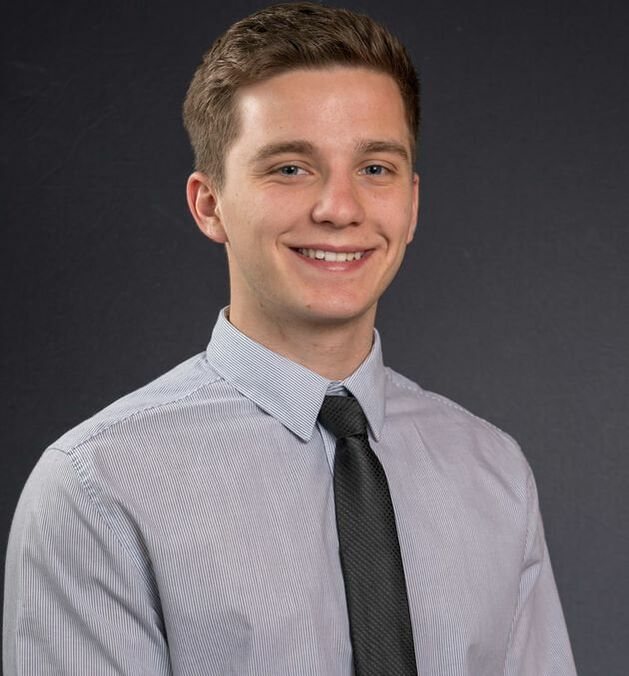
\includegraphics[width=1in,height=1.25in,clip,keepaspectratio]{a2.jpg}}]{Melvin Bosnjak} is a student, developer, and dog lover. He is currently studying Computer Engineering at the University of Utah, with an emphasis in software development. He studies a wide range of disciplines within software development such as networking, embedded systems, object oriented programming, computer organization, databases, web development and more. He enjoys taking on challenging projects in a team environment.
\end{IEEEbiography}

\begin{IEEEbiography}[{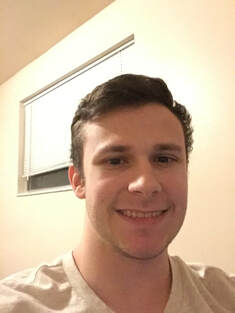
\includegraphics[width=1in,height=1.25in,clip,keepaspectratio]{a3.jpg}}]{Jaden Simon} is currently a computer engineering student at the University of Utah. Some of his favorite areas of study are hardware design, machine learning, and computer networking. In his free time, he enjoys learning about new things, hiking, and weight lifting.
\end{IEEEbiography}

\EOD

\end{document}
